\documentclass[9pt]{beamer}

%\usepackage{tikz}
\usepackage{amsmath}
\usepackage{amsfonts}
\usepackage{amssymb}
\usepackage{algorithm2e}
\usepackage{color, colortbl}
\usepackage{enumerate}
\usepackage{arydshln}
\usepackage{multirow}

\renewcommand{\figurename}{Fig}
\usetheme{uha}



%\theoremstyle{plain}
%  \newtheorem{theorem}{Theorem}
%  \newtheorem{lemma}{Lemma}
\newtheorem{corrolary}{Corollary}
\newtheorem{claim}{Claim}
\newtheorem{proposition}{Proposition}
\newtheorem{property}{Property}
%  \newtheorem{fact}{Fact}
%\theoremstyle{definition}
%  \newtheorem{definition}{Definition}
%  \newtheorem{example}{Example}
%\theoremstyle{remark}
\newtheorem{remark}{Remark}
\newtheorem{proviso}{Proviso}


\newcommand{\ccr}[1]{{\color{red}#1}}
\newcommand{\ccb}[1]{{\color{blue}#1}}
\newcommand{\ccp}[1]{{\color{purple}#1}}
\newcommand{\ccm}[1]{{\color{magenta}#1}}
\newcommand{\cco}[1]{{\color{orange}#1}}
\newcommand{\ccy}[1]{{\color{yellow}#1}}
\newcommand{\ccl}[1]{{\color{lime}#1}}
\newcommand{\ccc}[1]{{\color{cyan}#1}}
\newcommand{\ccg}[1]{{\color{gray}#1}}
\newcommand{\ccpk}[1]{{\color{pink}#1}}
\newcommand{\ccov}[1]{{\color{olive}#1}}



\begin{document}
	
%%//////////////////////////////////////////////////////////////////////////////////////////////%%1
	
    \title{Model-Agnostic Meta-Learning (MAML) }
    \subtitle{A Meta-Learning approach for Fast Adaptation of Deep Networks}
    \author{Yuyang Huang, Xuyang Zhao}
    \institute{School of Software, Shanghai Jiao Tong University}
    \date{\hspace{2em}}
    \frame{
    \titlepage
    }

%%//////////////////////////////////////////////////////////////////////////////////////////////%%1

\section{Introduction}


%%//////////////////////////////////////////////////////////////////////////////////////////////%%3
	\frame{
		\frametitle{Introduction: Meta-Learning}

		Meta learning = Learning to learn 

		* \ccr{Meta} + X $\longrightarrow$ X about X

		\centerline{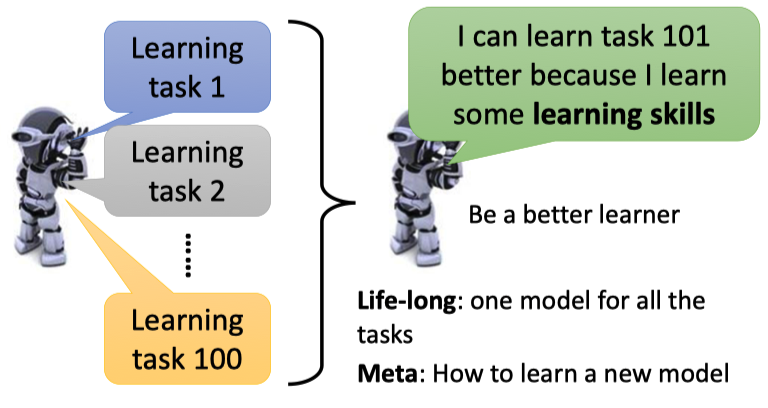
\includegraphics[width=1.0\textwidth]{figs/meta-ml.png}}
	}
	\frame{	
		\frametitle{Introduction: Meta-Learning Background}
		\textbf{A meta-learning model}
		\begin{itemize}
			\item learns from \ccb{past learning experience}				
			\item can learn \ccb{future tasks} \ccr{better} based on prior knowledge
			\item learns the learning function during the learning process
		\end{itemize}

		\textbf{Metrics for meta-learning}
		\begin{itemize}
			\item size of training-set for model convergence		
			\item robustness of model
			\item accuracy of the prediction
			\item etc...
		\end{itemize}
		
		}
%//////////////////////////////////////////////////////////////////////////////////////////////%%4
	\frame{
		\frametitle{Introduction: Few-shot Learning problem}
	
	\begin{definition}
		An \ccp{$st$-cut (cut)} is a partition \ccb{$(A, B)$} of the nodes with \ccb{$s\in A$} and \ccb{$t \in B$}.
	\end{definition}\pause

	\begin{definition}
 Its \ccp{capacity} is the sum of the capacities of the edges from \ccb{$A$} to \ccb{$B$}.
  \ccb{\[
\operatorname{cap}(A, B)=\sum_{e \text { out of } A} c(e)
\]}\vspace{-1em}
    \end{definition}\pause\bigskip


\centerline{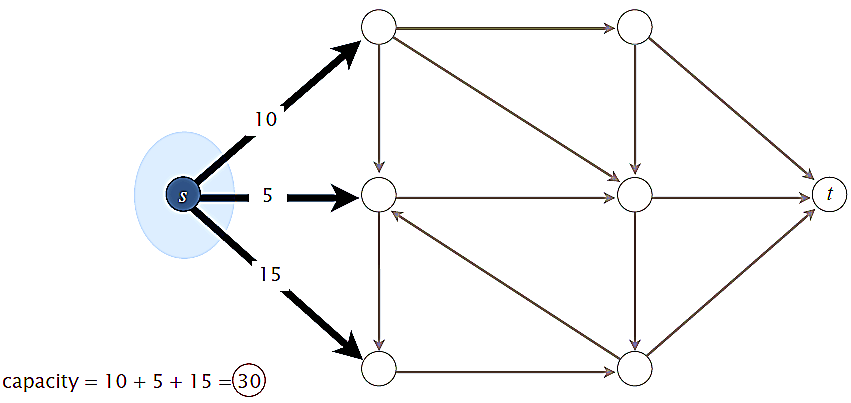
\includegraphics[width=0.65\textwidth]{figures/p4}}
	}
	%%%//////////////////////////////////////////////////////////////////////////////////////////////%%5
	\frame{
	\frametitle{Minimum-cut problem}
	\begin{definition}
		An \ccp{$st$-cut (cut)} is a partition \ccb{$(A, B)$} of the nodes with \ccb{$s\in A$} and \ccb{$t \in B$}.
	\end{definition}

	\begin{definition}
 Its \ccp{capacity} is the sum of the capacities of the edges from \ccb{$A$} to \ccb{$B$}.
  \ccb{\[
\operatorname{cap}(A, B)=\sum_{e \text { out of } A} c(e)
\]}\vspace{-1em}
    \end{definition}\bigskip	
	
	\centerline{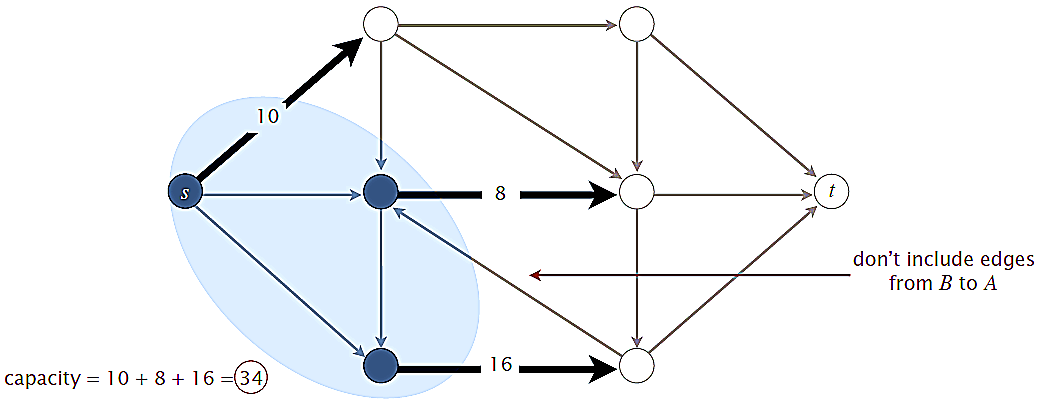
\includegraphics[width=0.7\textwidth]{figures/p5}}
}
	%%//////////////////////////////////////////////////////////////////////////////////////////////%%6

	\frame{
	\frametitle{Few-shot Learning problem}
	
    \cco{Min-cut problem.} Find a cut of minimum capacity.\bigskip\bigskip

	\centerline{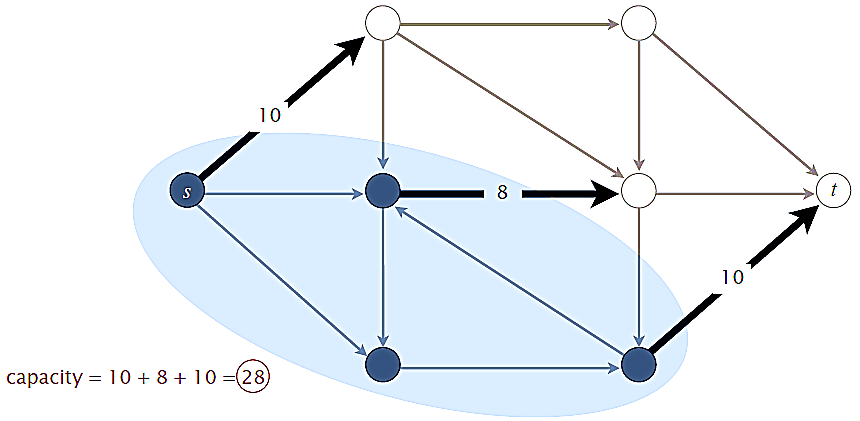
\includegraphics[width=0.6\textwidth]{figures/p6}}
}

	
%%//////////////////////////////////////////////////////////////////////////////////////////////%%7
		\frame{
		\frametitle{Few shot learning cases: Omniglot}
	Omniglot : Few-shot Classification
\begin{enumerate}[\color{blue} A.]
	\item $11~ (20+25 - 8 - 11 - 9 - 6)$
	\item $34 ~(8+11+9+6)$
	\item $45~ (20+ 25)$
	\item $79~	(20+ 25+ 8+ 11+ 9+ 6)$
\end{enumerate}	
\vspace{5mm}
	
	\centerline{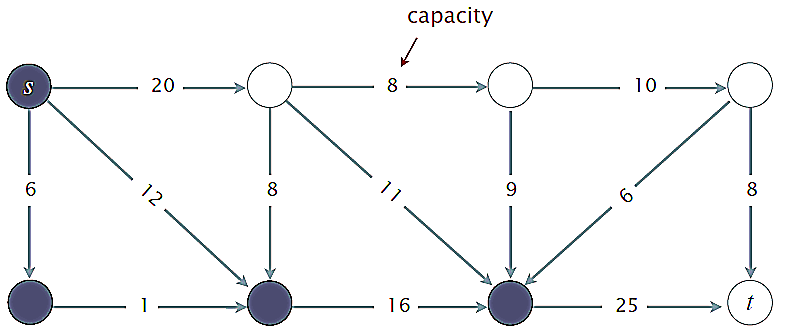
\includegraphics[width=0.8\textwidth]{figures/p7}}
	
}
	
	
	
	%%//////////////////////////////////////////////////////////////////////////////////////////////%%8
	\frame{
		\frametitle{Maximum-flow problem}
	\begin{definition}
		An \ccp{$st$-flow(flow)} \ccb{$f$} is a function that satisfies:
		\begin{itemize}
			\item For each \ccb{$e\in E$}: \hspace{2mm}  \ccb{$0 \leq f(e) \leq c(e)$}
			\item For each \ccb{$v\in V-\{s,t\}$}:  \ccb{$\sum\limits_{e \text { in to } v} f(e) \  =\sum\limits_{e \text { out of } v} f(e)$}
		\end{itemize}
	\end{definition}
	\bigskip

	\centerline{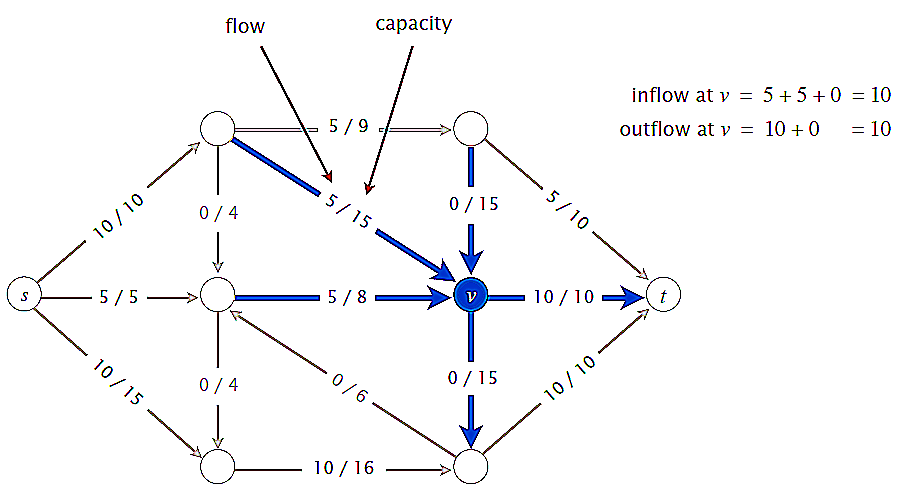
\includegraphics[width=0.8\textwidth]{figures/p8}}
	}
	
	%%//////////////////////////////////////////////////////////////////////////////////////////////%%9
	\frame{
		\frametitle{Maximum-flow problem}
		\begin{definition}
		An \ccp{$st$-flow(flow)} \ccb{$f$} is a function that satisfies:
		\begin{itemize}
			\item For each \ccb{$e\in E$}: \hspace{2mm}  \ccb{$0 \leq f(e) \leq c(e)$}
			\item For each \ccb{$v\in V-\{s,t\}$}:  \ccb{$\sum\limits_{e \text { in to } v} f(e) \  =\sum\limits_{e \text { out of } v} f(e)$}
		\end{itemize}
	\end{definition}
		\begin{definition}
		The \ccp{value}	of a flow \ccb{$f$} is: \ccb{$val(f)=\sum\limits_{e \text { out of } s} f(e)-\sum\limits_{e \text { in to } s} f(e)$}
		\end{definition}\smallskip
	
	\centerline{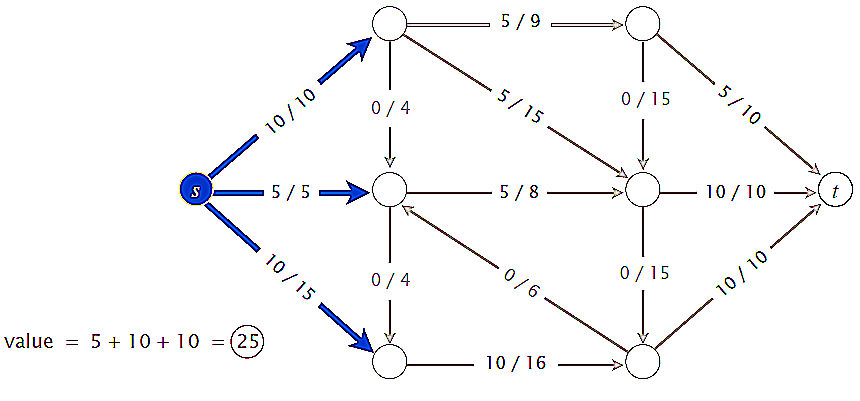
\includegraphics[width=0.7\textwidth]{figures/p9}}
	}
	
	
%%////////////////////////////////////////////////////////////////////////////////////////////%%10
	\frame{
	\frametitle{Maximum-flow problem}
	
    \cco{Max-flow problem.} Find a flow of maximum value.\bigskip\bigskip


	\centerline{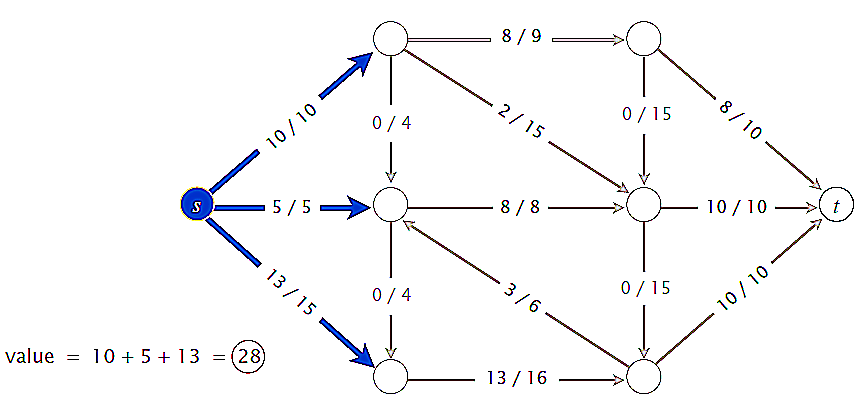
\includegraphics[width=0.7\textwidth]{figures/p10}}
}


\section{Model Agnostic Meta-Learning (MAML)}
	%
	%%//////////////////////////////////////////////////////////////////////////////////////////////%%12
	\frame{
		\frametitle{Toward a max-flow algorithm}
	\ccp{Greedy algorithm.}
	\vspace{-4mm}
		\begin{itemize}
			\item Start with \ccb{$f (e) = 0$} for each edge \ccb{$e \in E$}.
		\ccg{	\item Find an $s\rightsquigarrow t$ path $P$ where each edge has $f (e) < c(e)$.
			\item Augment flow along path $P$.
			\item  Repeat until you get stuck.}
		\end{itemize}\vspace{5mm}
	
	 	\centerline{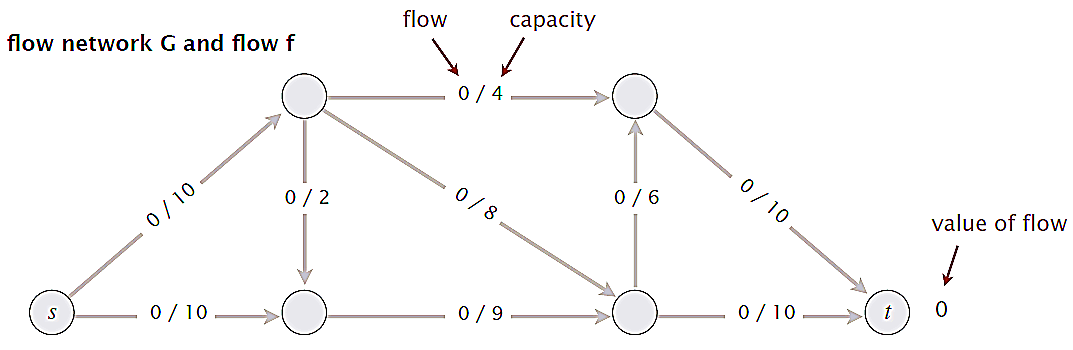
\includegraphics[width=\textwidth]{figures/p12}}
	}
	%
	%%//////////////////////////////////////////////////////////////////////////////////////////////%%13

\frame{
	\frametitle{Toward a max-flow algorithm}
	\ccp{Greedy algorithm.}
	\vspace{-4mm}
	\begin{itemize}
		\ccg{	\item Start with $f (e) = 0$ for each edge $e \in E$.}
		\item Find an \ccb{$s\rightsquigarrow t$} path \ccb{$P$} where each edge has \ccb{$f (e) < c(e)$}.
		\ccg{	\item Augment flow along path $P$.
			\item  Repeat until you get stuck.}
	\end{itemize}\vspace{5mm}
	
		\centerline{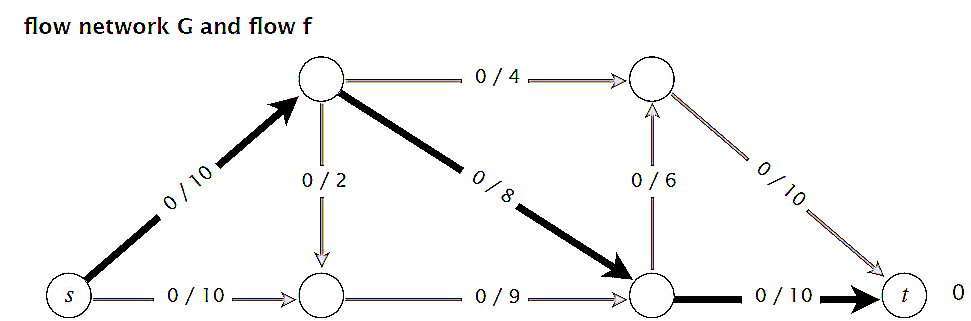
\includegraphics[width=\textwidth]{figures/p13}}
}
	%
	%%%%//////////////////////////////////////////////////////////////////////////////////////////////%%14
	%
\frame{
	\frametitle{Toward a max-flow algorithm}
	\ccp{Greedy algorithm.}
	\vspace{-4mm}
	\begin{itemize}
		\ccg{	\item Start with $f (e) = 0$ for each edge $e \in E$.
		\item Find an $s\rightsquigarrow t$ path $P$ where each edge has $f (e) < c(e)$.}
		\item Augment flow along path \ccb{$P$}.
		\ccg{	\item  Repeat until you get stuck.}
	\end{itemize}\vspace{5mm}
	
		\centerline{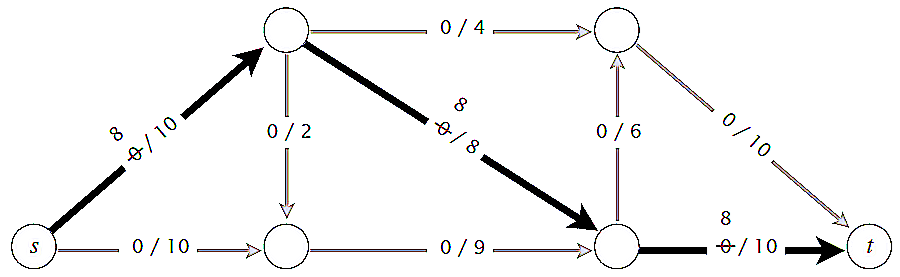
\includegraphics[width=\textwidth]{figures/p14}}
}
	%%%//////////////////////////////////////////////////////////////////////////////////////////////%%15
	
\frame{
	\frametitle{Toward a max-flow algorithm}
	\ccp{Greedy algorithm.}
	\vspace{-4mm}
	\begin{itemize}
		\ccg{	\item Start with $f (e) = 0$ for each edge $e \in E$.
			\item Find an $s\rightsquigarrow t$ path $P$ where each edge has $f (e) < c(e)$.
		\item Augment flow along path $P$.}
			\item  Repeat until you get stuck.
	\end{itemize}\vspace{3mm}
	
		\centerline{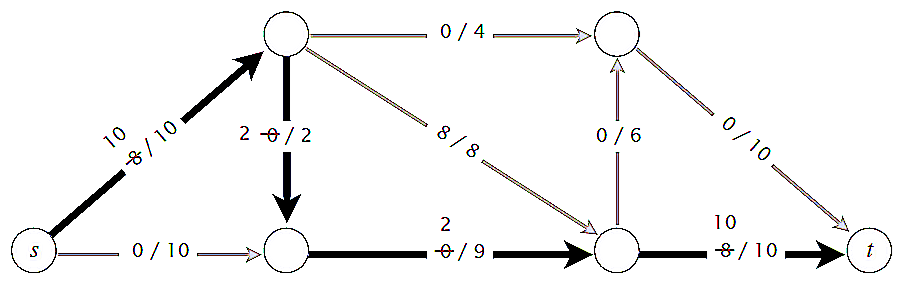
\includegraphics[width=\textwidth]{figures/p15}}
}
	%%%%//////////////////////////////////////////////////////////////////////////////////////////////%%16
   \frame{
	\frametitle{Toward a max-flow algorithm}
	\ccp{Greedy algorithm.}
	\vspace{-4mm}
	\begin{itemize}
		\ccg{\item Start with $f (e) = 0$ for each edge $e \in E$.
			\item Find an $s\rightsquigarrow t$ path $P$ where each edge has $f (e) < c(e)$.
			\item Augment flow along path $P$.}
		\item  Repeat until you get stuck.
	\end{itemize}\vspace{5mm}

	
		\centerline{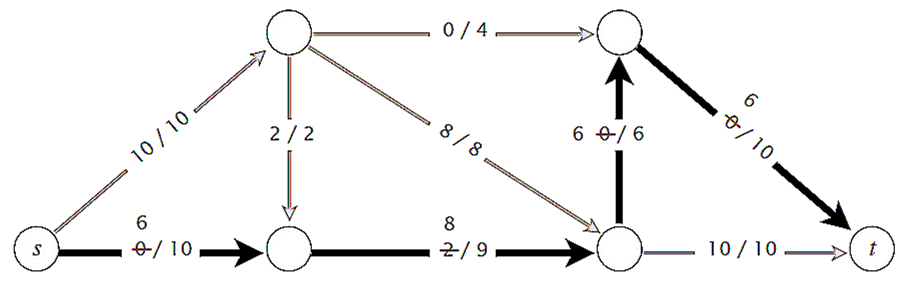
\includegraphics[width=\textwidth]{figures/p16}}
}
	%%%%//////////////////////////////////////////////////////////////////////////////////////////////%%17
\frame{
	\frametitle{Toward a max-flow algorithm}
	\ccp{Greedy algorithm.}
	\vspace{-4mm}
	\begin{itemize}
			\item Start with \ccb{$f (e) = 0$} for each edge \ccb{$e \in E$}.
			\item Find an \ccb{$s\rightsquigarrow t$} path \ccb{$P$} where each edge has \ccb{$f (e) < c(e)$}.
			\item Augment flow along path \ccb{$P$}.
		\item  Repeat until you get stuck.
	\end{itemize}
\bigskip

	
		\centerline{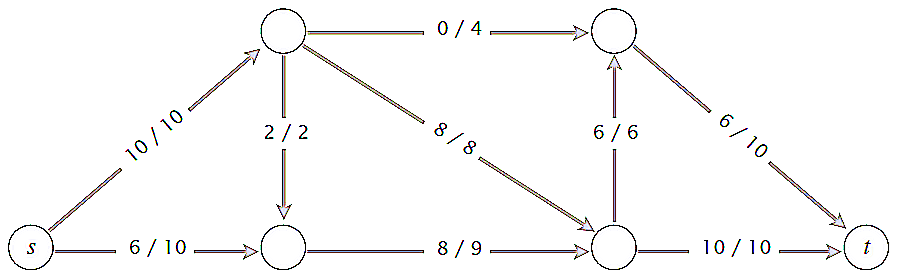
\includegraphics[width=\textwidth]{figures/p17}}
}
%%%%//////////////////////////////////////////////////////////////////////////////////////////////%%18

  \frame{
	\frametitle{Toward a max-flow algorithm}
	\ccp{Greedy algorithm.}
	\vspace{-4mm}
	\begin{itemize}
			\item Start with \ccb{$f (e) = 0$} for each edge \ccb{$e \in E$}.
			\item Find an \ccb{$s\rightsquigarrow t$} path \ccb{$P$} where each edge has \ccb{$f (e) < c(e)$}.
			\item Augment flow along path \ccb{$P$}.
		\item  Repeat until you get stuck.
	\end{itemize}
\bigskip
	
		\centerline{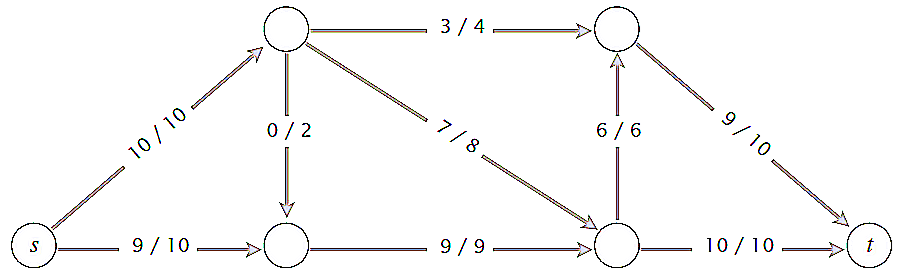
\includegraphics[width=\textwidth]{figures/p18}}
}
	
%%%%//////////////////////////////////////////////////////////////////////////////////////////////%%19

	\frame{
    \frametitle{Why the greedy algorithm fails}
		\ccr{Q.} Why does the greedy algorithm fail?\pause

		\ccc{A.} Once greedy algorithm increases flow on an edge, it never decreases it.
		\pause\smallskip
		
		\cco{Ex.} Consider flow network \ccb{$G$}.	\vspace{-3mm}
		\begin{itemize}
			\item The unique max flow has \ccb{$f^*(v,w)=0$}.
			\item Greedy algorithm could choose \ccb{$s\rightarrow v\rightarrow w \rightarrow t$} as first augmenting path.
		\end{itemize}\smallskip
		
		\centerline{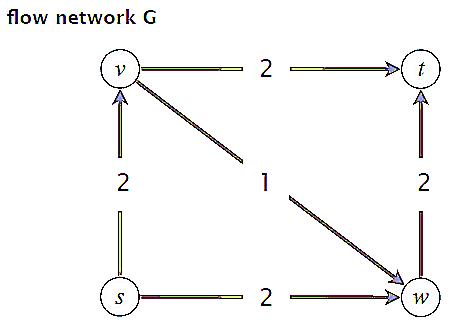
\includegraphics[width=0.4\textwidth]{figures/p19}}\pause
		
	\cco{Bottom line.} Need some mechanism to \ccr{undo} a bad decision.	
	}
	%%%%//////////////////////////////////////////////////////////////////////////////////////////////%%20
	\frame{
		\frametitle{Residual network}
		\vspace{2mm}
	\begin{columns}
		\begin{column}{6cm}
			\ccp{Original edge} \ccb{$e=(u,v)\in E$}.
			\begin{itemize}
				\item Flow \ccb{$f(e)$}.
				\item Capacity \ccb{$c(e)$}
			\end{itemize}	
		\vspace{3mm}
		
			\ccp{Reverse edge}  \ccb{$e^{\text { reverse }}=(v, u)$}
			\begin{itemize}
				\item	\cco{Undo} flow sent.
			\end{itemize}	
		
		\end{column}
	
		\begin{column}{4cm}
	\centerline{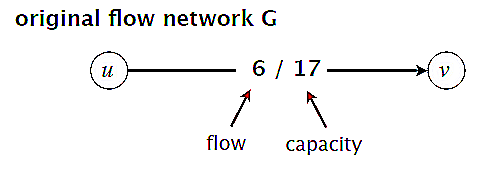
\includegraphics[width=\textwidth]{figures/p20}}
	\end{column}
	\end{columns}
\bigskip\pause
	\begin{columns}
		
	\begin{column}{6cm}
\ccp{Residual capacity}
\ccb{$$
c_{f}(e)=\left\{\begin{array}{ll}{c(e)-f(e)} & {\text { if } e \in E} \\ {f(e)} & {\text { if } e^{\text { reverse }} \in E}\end{array}\right.
$$}
  \end{column}
	
	\begin{column}{4cm}
		\centerline{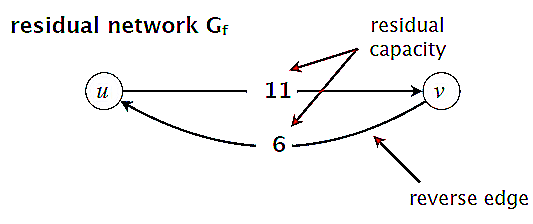
\includegraphics[width=\textwidth]{figures/p20_2}}
	\end{column}
\end{columns}


\ccp{Residual network} \ccb{$G_f=(V,E_f,s,t,c_f)$} 	%$ \color{red}\begin{array}{l}
%\text{\tiny edges with positive}\\[-2mm]
%\text{\tiny residual capacity}\\
%\swarrow\\
%\end{array} $ 	\vspace{-4mm}
\begin{itemize}
		\vspace{-4mm}
	\item \ccb{$E_{f}=\{e : f(e)<c(e)\} \cup\left\{e^{\text { reverse }} : f(e)>0\right\}$}.	%$ \color{red}\begin{array}{l}
%	\text{\tiny where flow on a reverse edge}\\[-2mm]
% \quad	\text{\tiny negates flow on}\\[-2mm]
%	\text{\tiny corresponding forward edge}\\
%	\swarrow\\
%	\end{array} $
% \vspace{-2mm}
	\item Key property: \ccb{$f'$} is a flow in \ccb{$G_f$} iff \ccb{$f+f'$} is a flow in \ccb{$G$}
\end{itemize}
	}
	%%
%%%%//////////////////////////////////////////////////////////////////////////////////////////////%%21

\frame{
	\frametitle{Augmenting path}
	\begin{definition}
		An \ccp{augmenting path} is a simple \ccb{$s\rightsquigarrow t$} path in the residual network \ccb{$G_f$}.
	\end{definition}\pause

  \begin{definition}
	The \ccp{bottleneck capacity} of an augmenting path \ccb{$P$} is the minimum residual capacity of any edge in \ccb{$P$}.	
   \end{definition}
  }

%%%%//////////////////////////////////////////////////////////////////////////////////////////////%%21

\frame{
	\frametitle{Augmenting path}

    \cco{Key Property.}
    Let \ccb{$f$} be a flow and let \ccb{$P$} be an augmenting path in \ccb{$G_f$}. After calling \ccb{$f'\leftarrow\mathtt{Augment}(f,c,P)$}, the resulting \ccb{$f'$} is a flow and \ccb{$val(f')=val( f )+bottleneck(G_f, P)$}.\pause

    \begin{exampleblock}{}
   % \scalebox{0.9}{
    \begin{algorithm}[H]
        \SetKwData{x}{x}\SetKwData{y}{y}\SetKwData{z}{z}
        \SetKwFunction{Au}{\sc Augment}\SetKwFunction{Return}{\sc Return}\SetKwFunction{Init}{\sc Initialize}
        \SetKwInOut{Input}{input}\SetKwInOut{Output}{output}
     \Au{$f$,$c$,$P$}
     \BlankLine
     $\delta \leftarrow$ bottleneck capacity of augmenting path P\;
     \For{each edge $e\in P$}{
       \lIf{$(e\in E)$}{$f(e)\leftarrow f(e)+\delta$}
      \Else{$f\left(e^{\text { reverse }}\right) \leftarrow f\left(e^{\text { reverse }}\right)-\delta$}
      }
      \Return $f$\;
     \end{algorithm}
     \end{exampleblock}

     }
	%%
	%%%%//////////////////////////////////////////////////////////////////////////////////////////////%%22
	%
	\frame{
		\frametitle{Network flow: quiz 2}
	Which is the augmenting path of highest bottleneck capacity?
	\begin{enumerate}\color{blue}
		\item $A \rightarrow F \rightarrow G \rightarrow H$
		\item $A \rightarrow B \rightarrow C \rightarrow D \rightarrow H$
		\item $A \rightarrow F \rightarrow B \rightarrow G \rightarrow H$
		\item $A \rightarrow F \rightarrow B \rightarrow G \rightarrow C \rightarrow D \rightarrow H$
	\end{enumerate}	\vspace{3mm}
		\centerline{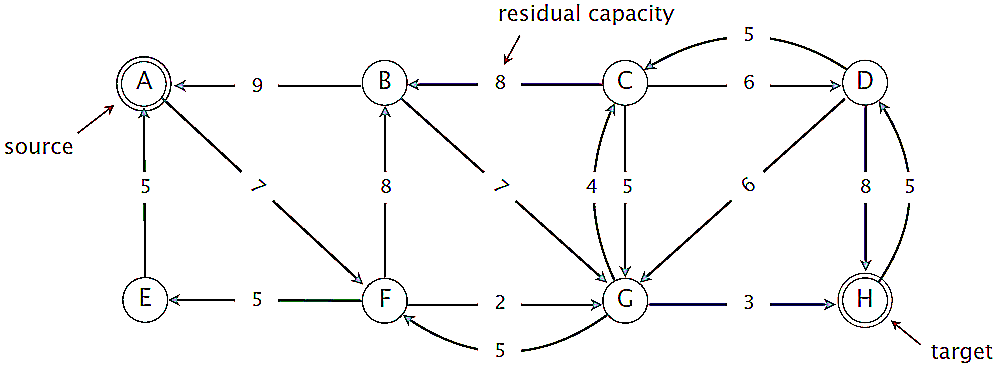
\includegraphics[width=0.8\textwidth]{figures/p22}}
	}
	%%
	%%%%//////////////////////////////////////////////////////////////////////////////////////////////%%23
	\frame{
		\frametitle{Ford–Fulkerson algorithm}
		\ccp{Ford–Fulkerson augmenting path algorithm.}
		\vspace{-3mm}
		\begin{itemize}
		\item Start with \ccb{$f (e) = 0$} for each edge \ccb{$e \in E$}.
		\item Find an \ccb{$s\rightsquigarrow t$} path \ccb{$P$}  in the residual network \ccb{$G_f$}.
		\item Augment flow along path \ccb{$P$}.
		\item  Repeat until you get stuck.
		\end{itemize}
	\pause

	\begin{exampleblock}{}
    \begin{algorithm}[H]
        \SetKwData{x}{x}\SetKwData{y}{y}\SetKwData{z}{z}
        \SetKwFunction{FF}{\sc Ford–Fulkerson}\SetKwFunction{Return}{\sc Return}\SetKwFunction{Init}{\sc Initialize}
        \SetKwFunction{Up}{\sc Update}\SetKwFunction{Au}{\sc Augment}
        \SetKwInOut{Input}{input}\SetKwInOut{Output}{output}
     \FF{$G$}
     \BlankLine
     \For{each edge $e \in E$}{$f(e)\leftarrow 0$}
     $G_f\leftarrow $ residual network of $G$ with respect to flow $f$\;

     \While{there exists an $s\rightsquigarrow t$ path $P$ in $G_f$}{
      $f\leftarrow$ \Au{$f$,$c$,$P$}\;
      \Up{$G_f$}\;
      }
      \Return $f$\;
     \end{algorithm}
     \end{exampleblock}

	}
	%%%%//////////////////////////////////////////////////////////////////////////////////////////////%%24

	\section{Algorithms}

	%%%%//////////////////////////////////////////////////////////////////////////////////////////////%%25
	
	\frame{
		\frametitle{Relationship between flows and cuts}
		\begin{lemma}
		Let \ccb{$f$} be any flow and let \ccb{$(A,B)$} be any cut. Then, the value of the flow \ccb{$f$} equals the net flow across the cut \ccb{$(A,B)$}.	
		\ccb{\begin{equation*}
	v a l(f)=\sum\limits_{\text { out of } A} f(e)-\sum\limits_{e \text { in to } A} f(e)
		\end{equation*}}
    \end{lemma}
	
	\bigskip
   	\centerline{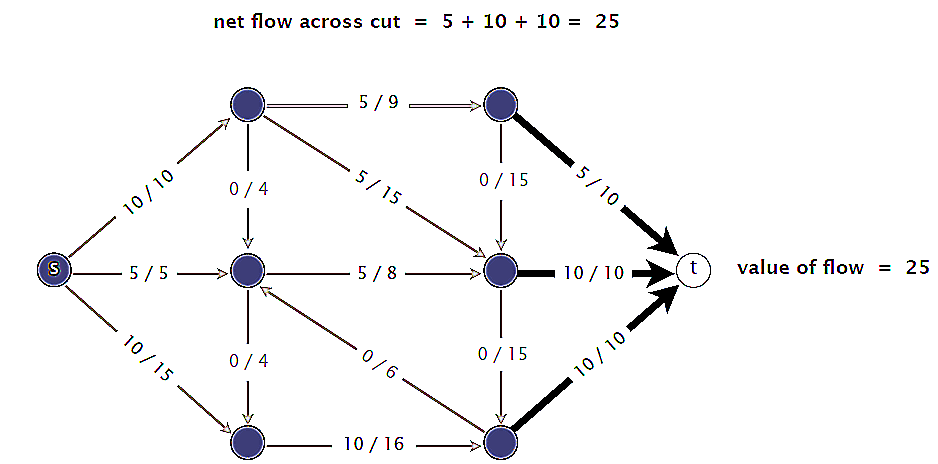
\includegraphics[width=0.8\textwidth]{figures/p25}}
	}


%%//////////////////////////////////////////////////////////////////////////////////////////////%%36
	
    \section{MeLU: MAML for Cold-Start Recommendation}
	
%%//////////////////////////////////////////////////////////////////////////////////////////////%%37
	%%
	%%
	\frame{
		\frametitle{Cold-Start Recommendation problem}

		\ccp{Recommendation.} \\
		Companies use recommendation systems to deliver personalized contents and sell products. 
		
		\begin{columns}
			\begin{column}{8cm}
				\centerline{
\includegraphics[width=0.3\textwidth]{figs/tiktok.png}}		
			\end{column}
			\begin{column}{4cm}
				\centerline{
\includegraphics[width=0.3\textwidth]{figs/taobao.jpeg}}	
			\end{column}
		\end{columns} 
		\pause
		
		\ccp{Cold-Start problem.} \\
		Modern recommendation systems use \ccp{Machine Learning} approach to provide \ccp{customized} user-experience.
		Recommendation using ML is hard when \#users and \#items are still small. (\ccr{A Cold-Start}).

		\pause
		
		\begin{definition}
			\ccm{Few-Shot Learning} 
			\begin{itemize}
				\item Few-shot learning is the problem of making predictions based on a limited number of samples.
			\end{itemize}
		\end{definition}	
	}

%%//////////////////////////////////////////////////////////////////////////////////////////////%%37

	\frame{
		\frametitle{MAML for cold-start recommendation}
		
		\ccr{User Preference Estimator.} the model that estimate users' preference for certain item.
		\centerline{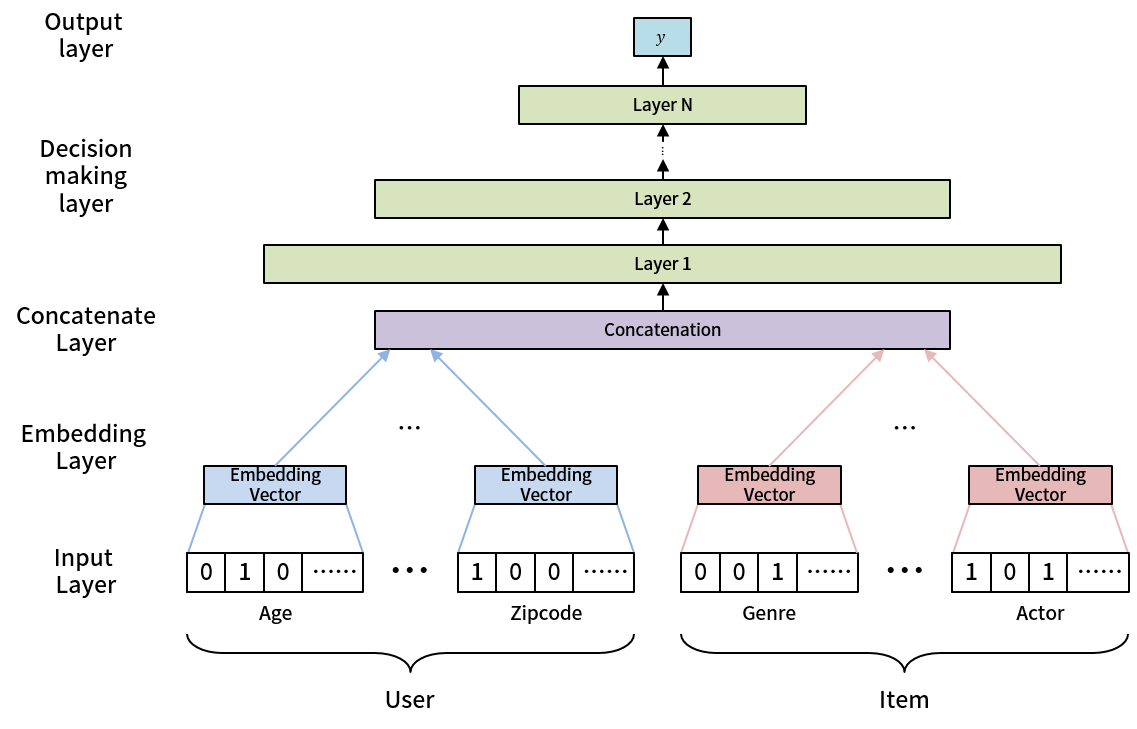
\includegraphics[width=1\textwidth]{figs/melu-pref.png}}

	}
	%%
	%%%%//////////////////////////////////////////////////////////////////////////////////////////////%%38
	
	\frame{
		\frametitle{User Preference Estimator.}
		
		\begin{block}{Model layers of UPE} 
			\begin{itemize}
				\item \textbf{Input Layer} : get input information, including user's profile and item's information \pause
				\item \textbf{Embedding Layer} : Embedding input information into embedding vectors. \pause
				\item \textbf{Concatenate Layer}: Concatenate different vectors into one big vector. \pause
				\item \textbf{Decision-Making Layers}: transform concatenated vector into characteristics  \pause
				\item \textbf{Output Layer}: get output information in the form of preference probability, rating, dwell time,etc.
			\end{itemize}
		\end{block} \pause
		
		This typical user preference estimator takes users' content and item content as input, and output preference prediction.
	}

%%%%//////////////////////////////////////////////////////////////////////////////////////////////%%46
	
	\frame{
		\frametitle{Meta-learned User Preference Estimator}
		
		\textbf{How to improve estimator's performance when \ccr{training set is small ?}}
		
		Apply MAML's approach to UPE ! \pause

		\centerline{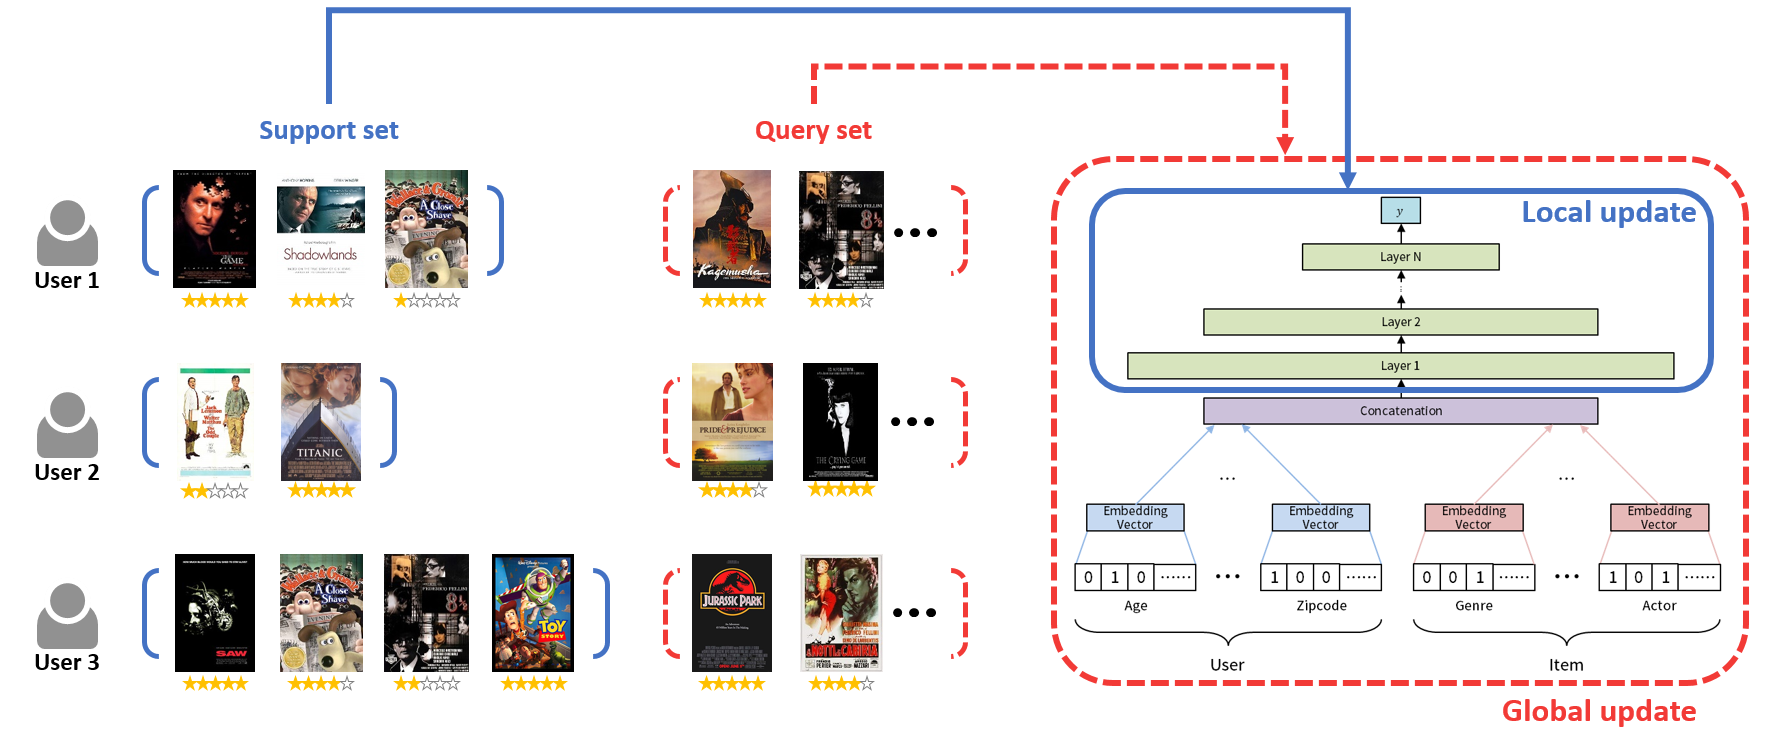
\includegraphics[width=1\textwidth]{figs/meta-upe.png}}

	}

%%%%//////////////////////////////////////////////////////////////////////////////////////////////%%46
	
\frame{
	\frametitle{Meta-learned User Preference Estimator}
	
	\begin{block}{Loss function of UPE}
		$\mathcal{L}_i = \frac{1}{\left | H_i \right | } \sum_{j\in H_i} (y_{ij} - \hat{y}_{ij})^2 $
	\end{block} \pause
	
	\centerline{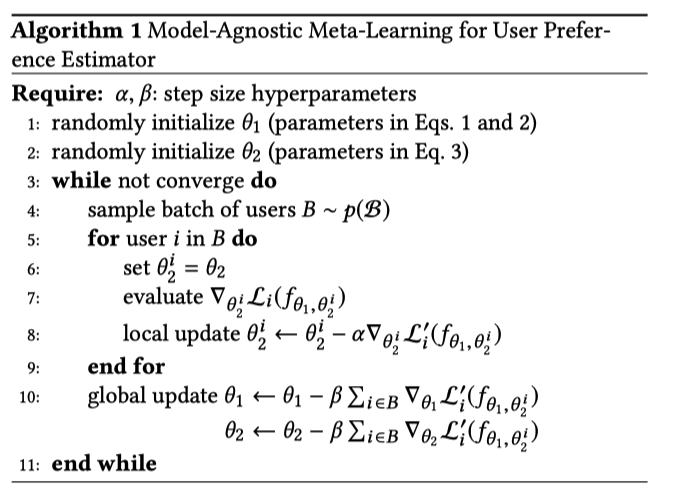
\includegraphics[width=0.8\textwidth]{figs/melu-alg.png}}
}

%%%%//////////////////////////////////////////////////////////////////////////////////////////////%%46
	
\frame{
	\frametitle{Evidence Candidate Selection}

	\begin{block}{Evidence Candidates}
		\ccr{Evidence candidate} is a set of items that are presented to a new user, so that the model can get a quick understand of user's general preference for products.
	\end{block} \pause

	\textbf{We can user evidence candidates to}
	\begin{itemize}
		\item quickly understand user's preference by doing a survey on \ccb{evidence candidate}
		\item collaborate with Meta-learning approach to further improve few-shot accuracy.
	\end{itemize}
	\centerline{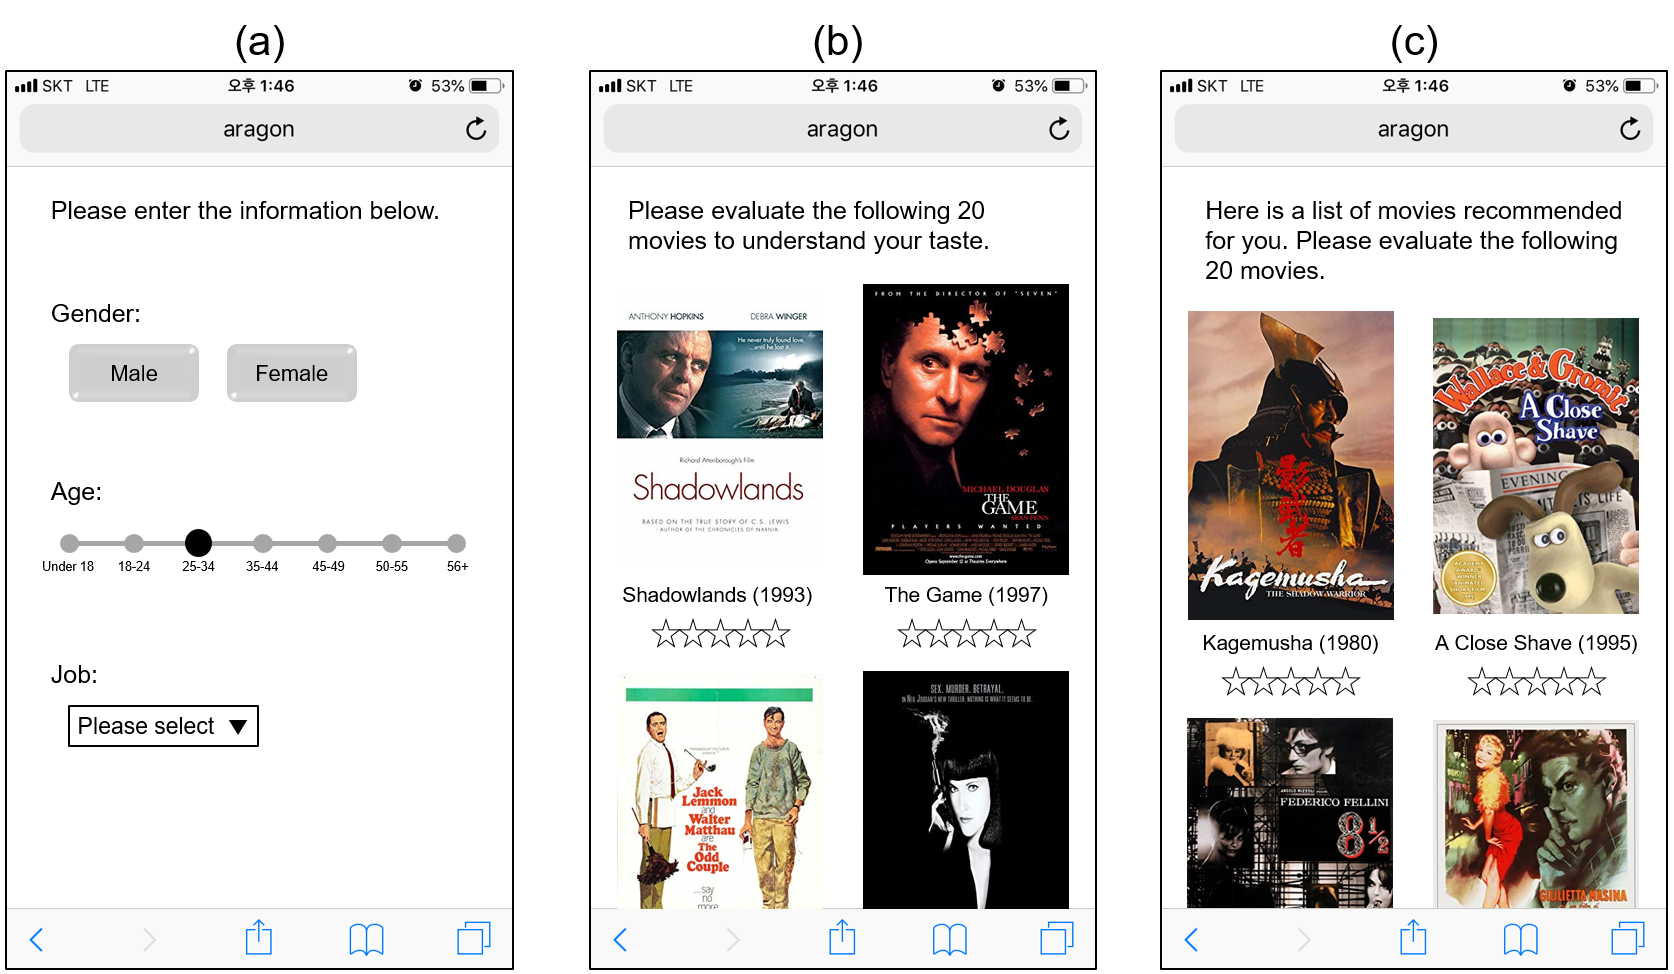
\includegraphics[width=0.5\textwidth]{figs/melu-candi.png}}
	
}

%%%%//////////////////////////////////////////////////////////////////////////////////////////////%%46
	
\frame{
	\frametitle{Evaluations}

	MeLU is able to predict well with only a few input.

	\textbf{The MAE of MeLU on the MovieLens and Bookcrossing datasets}
	\centerline{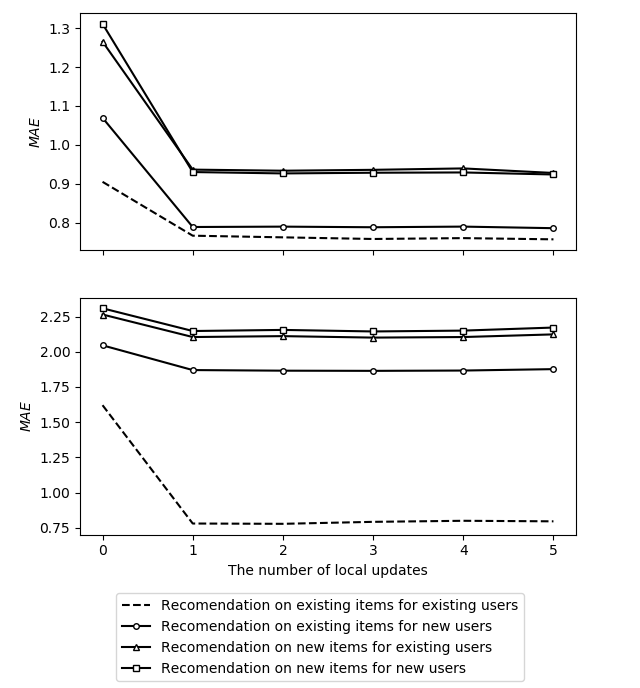
\includegraphics[width=1\textwidth]{figs/melu-eva.png}}
	
}
%%%%//////////////////////////////////////////////////////////////////////////////////////////////%%46
	
\frame{
	\frametitle{What can we learn from MeLU?}

	\textbf{MAML is a general approach}
	\begin{itemize}
		\item we can apply MAML to any gradient-based model.
		\item meta-learning approach can be useful in everyday tasks.
	\end{itemize}
	
	\textbf{Field-specific approach can be taken}
	\begin{itemize}
		\item to improve learning performance
		\item to focus on important metrics
	\end{itemize}

	
}
%%%%//////////////////////////////////////////////////////////////////////////////////////////////%% 7 pages

	\section{More on meta-learning }

%%%%//////////////////////////////////////////////////////////////////////////////////////////////%%48
	%%
	\frame{
		\frametitle{Meta-learning is not only MAML}
		\textbf{MAML takes a optimization-based approach}
		\begin{itemize}
			\item MAML fundamentally produce a weight initialization, it learns a good initial parameter   \pause
			\item not introduce any learned parameters more meta-learning  \pause
			\item not actually learn any more general knowledge like \ccb{"how to learn a brand new task?"}
		\end{itemize} \pause

		\textbf{There actually exists other approaches...}
		\begin{itemize}
			\item Model-based : a new model designed specifically for fast learning, which in its nature updates parameters rapidly. May use RNN and memory techniques. \pause
			\item Metric-based : derive problem-dependent good metrics, to facilitate problem solving.
		\end{itemize} 
		
	}
	
	
%%%%//////////////////////////////////////////////////////////////////////////////////////////////%% 3
%%
\frame{
	\frametitle{Beyond Gradient Descent}
	\textbf{How to meta-learn other metrics on models other than gradient-based.}

	\centerline{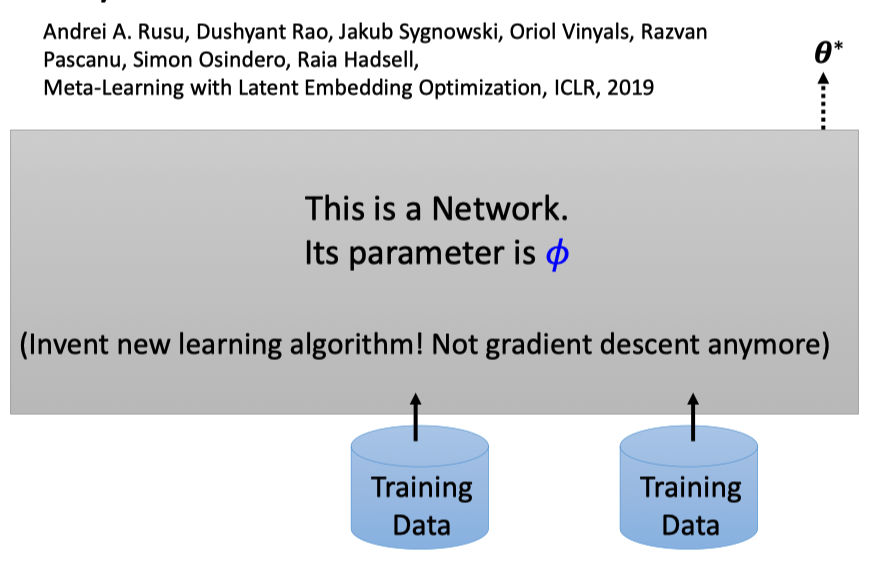
\includegraphics[width=1\textwidth]{figs/beyond-gd.png}}
}
%%%%//////////////////////////////////////////////////////////////////////////////////////////////%% 3
%%
	\frame{
		\frametitle{Meta-learning is a huge field}
		\textbf{Matching network}
		Matching network is one of the \ccr{metric-based} meta-learning works that targeting k-shot classification problems.

		\centerline{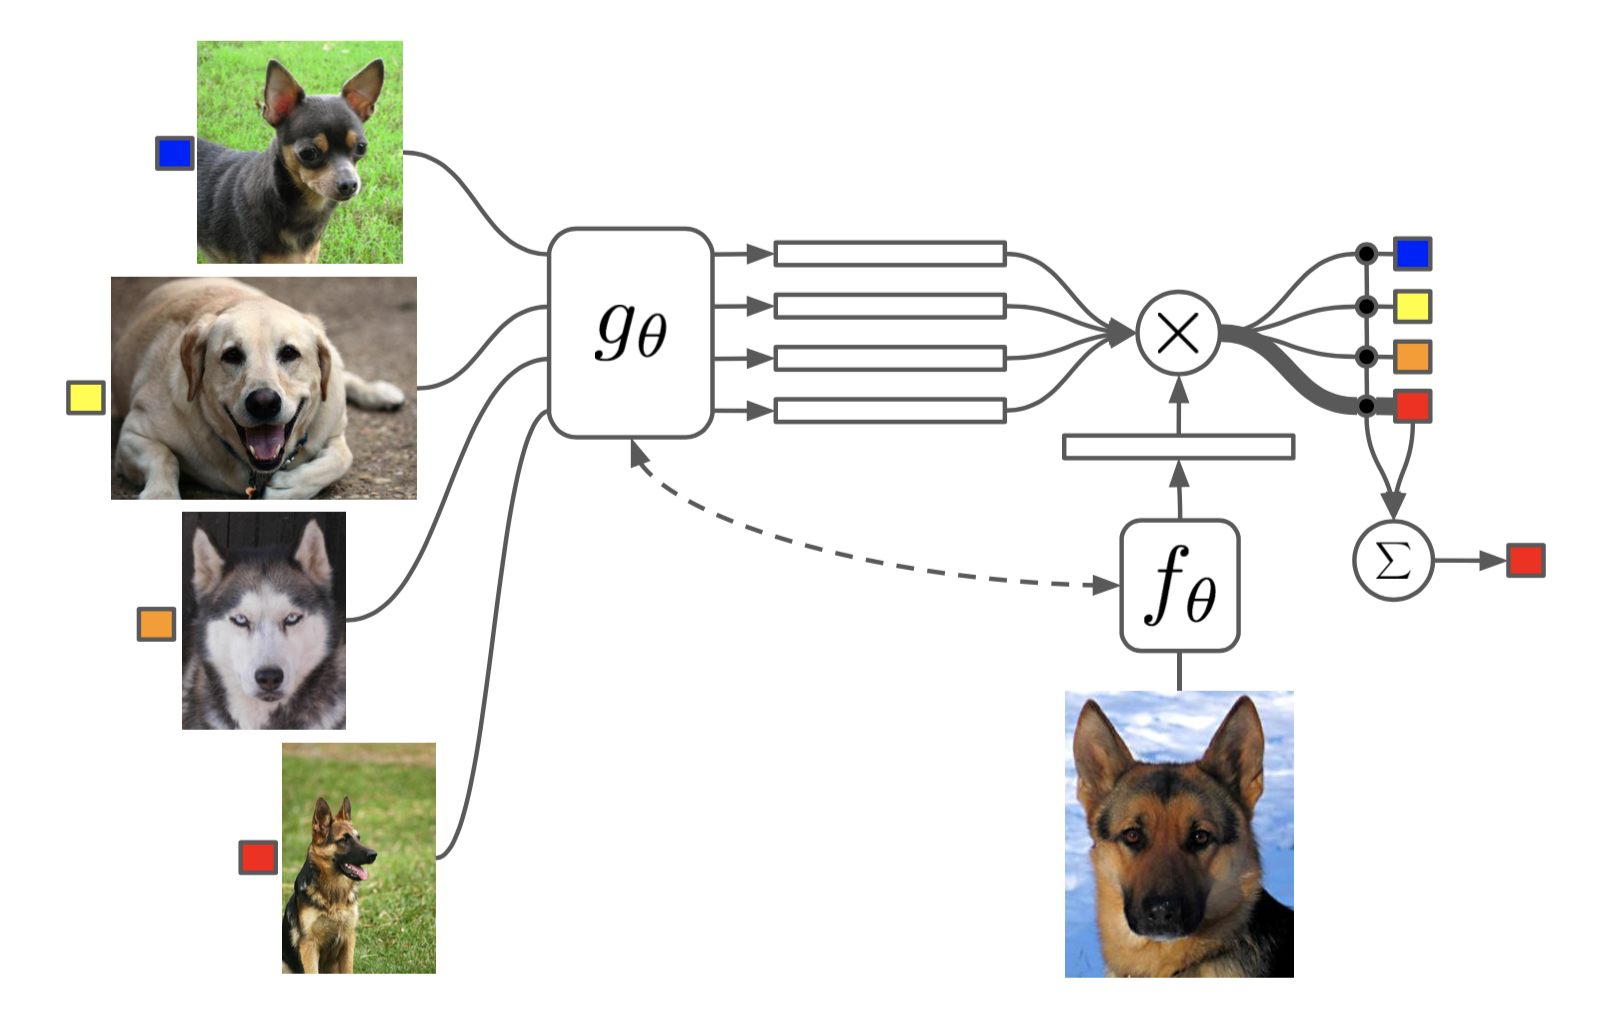
\includegraphics[width=1\textwidth]{figs/matching-networks.png}}
	}
	
%%%%//////////////////////////////////////////////////////////////////////////////////////////////%% 3
%%
	\frame{
		\frametitle{Meta-learning is a huge field}
		\textbf{Meta network}
		Meta Networks , short for MetaNet, is a \ccr{model-based} meta-learning model with architecture and training process designed for \ccpk{rapid generalization across tasks}.
		me
		\centerline{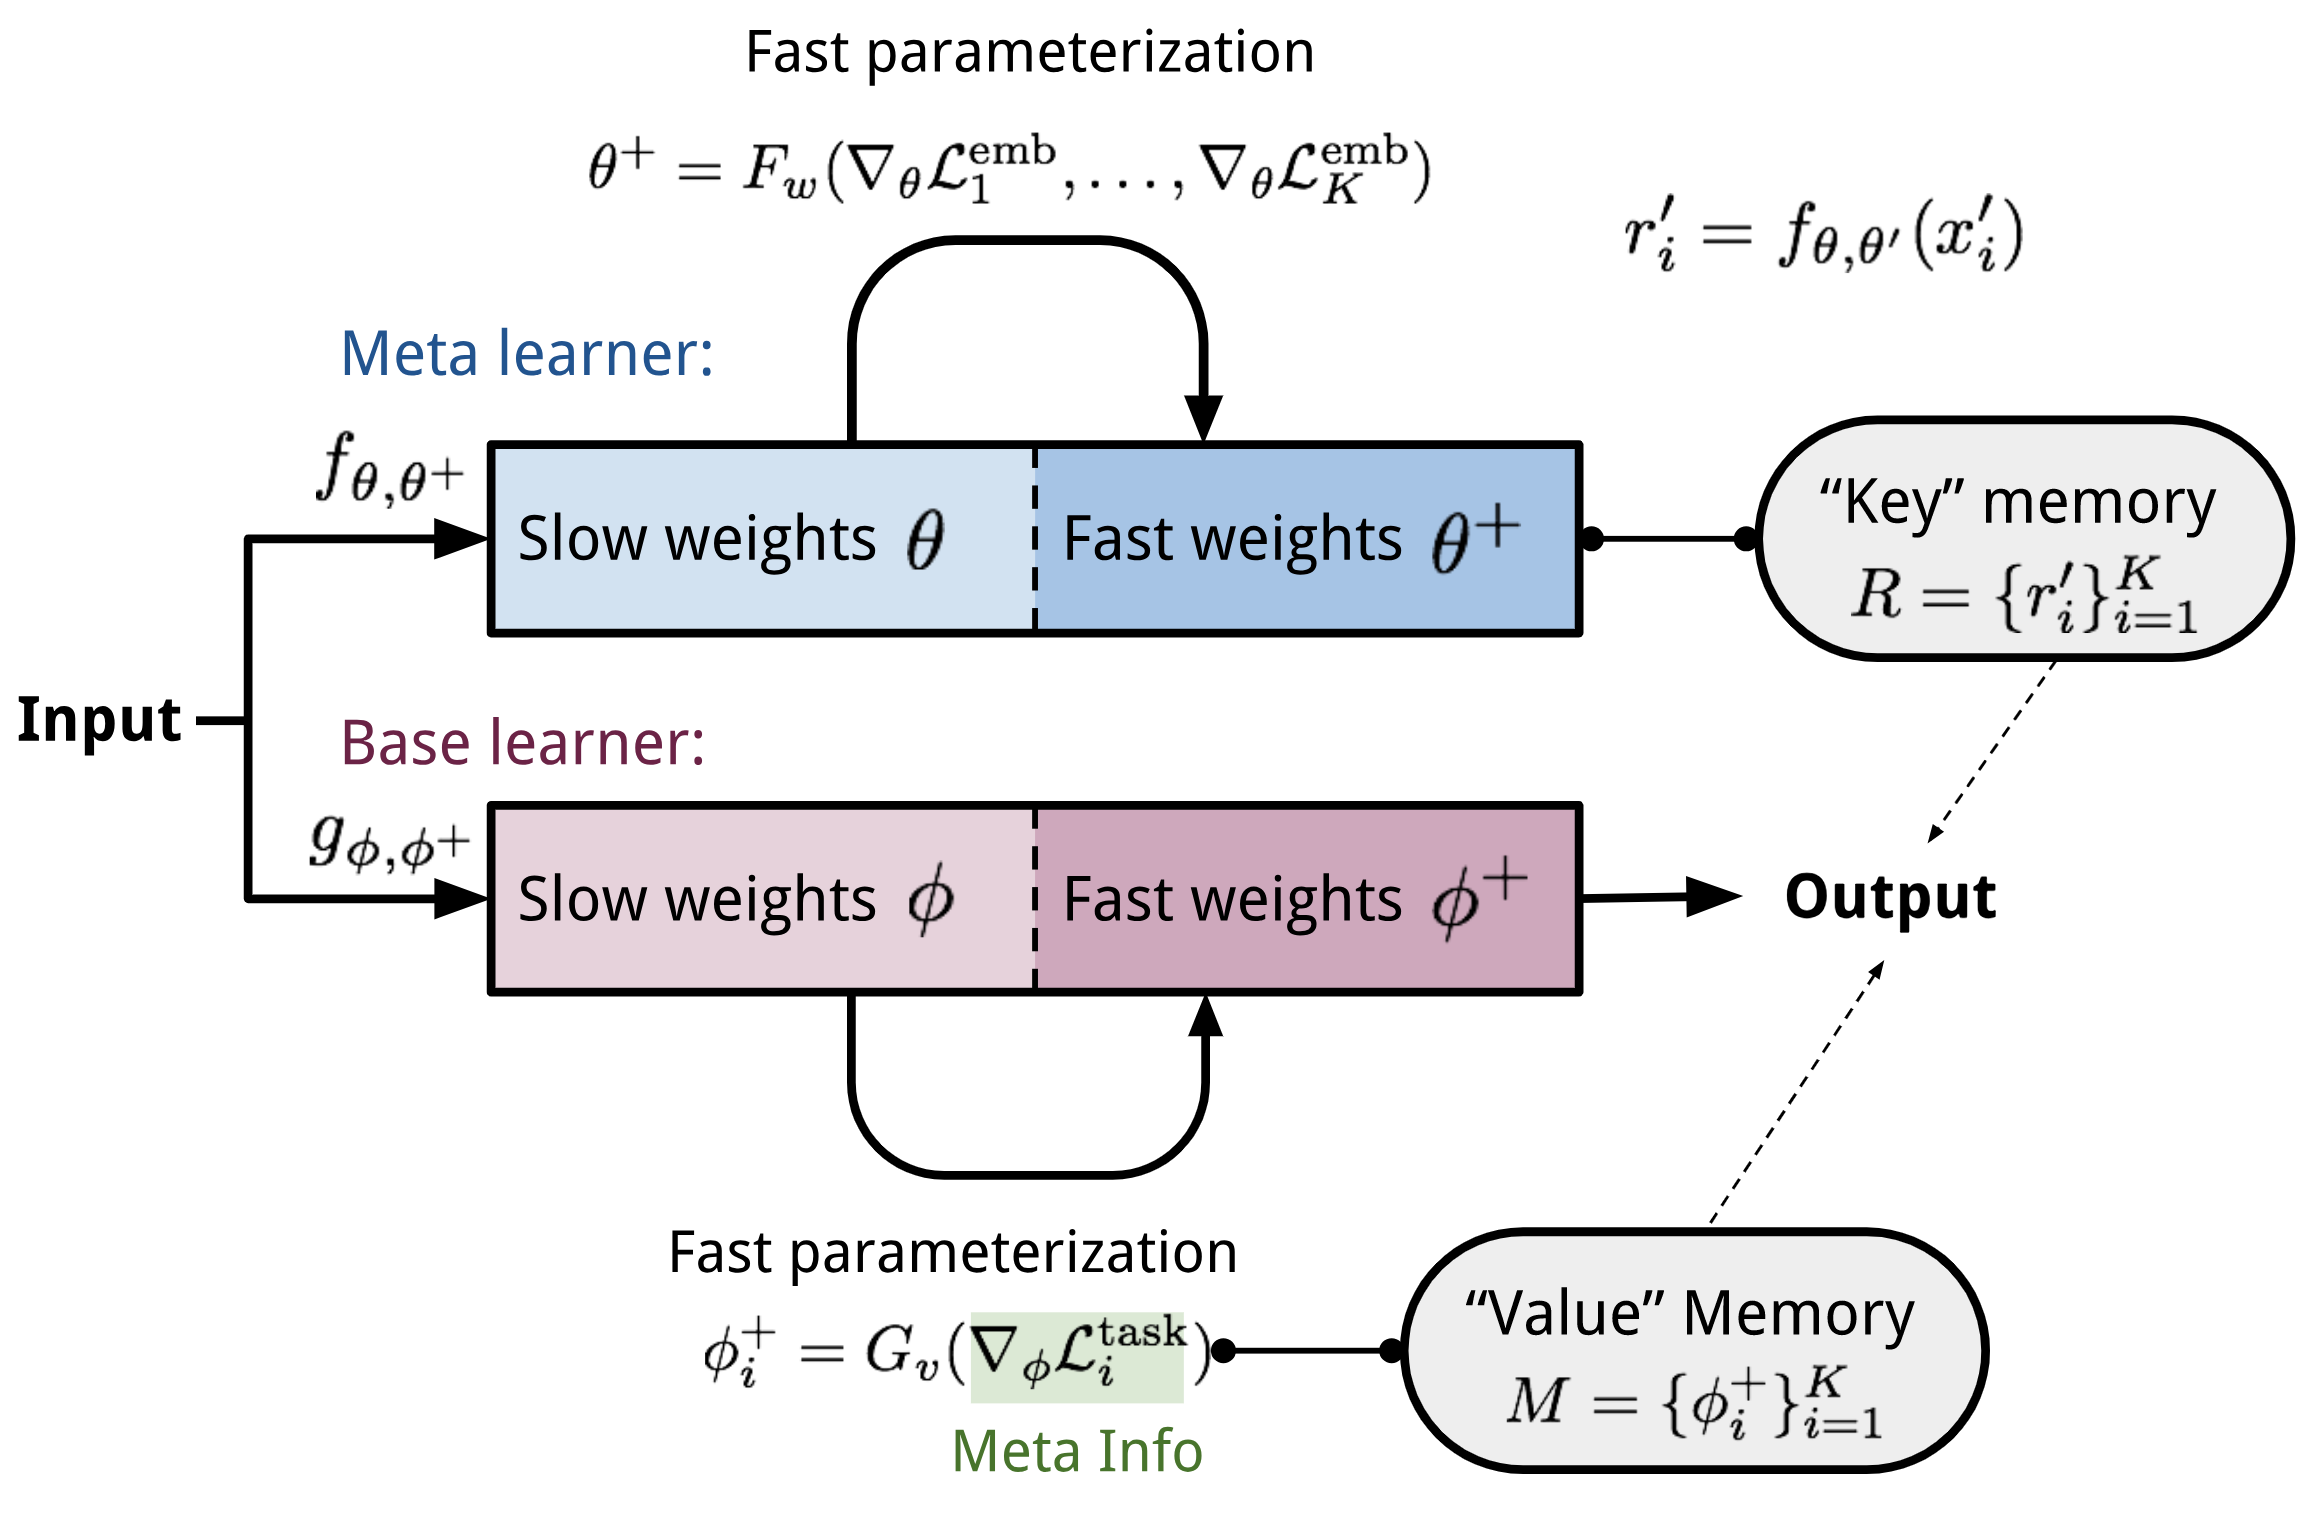
\includegraphics[width=1\textwidth]{figs/meta-network.png}}
	}

%%%%//////////////////////////////////////////////////////////////////////////////////////////////%%48
%%
\frame{
	\frametitle{Meta-learning is a huge field}
	\textbf{Meta-learning Landscape}
	Overview of the meta-learning landscape including algorithm design (meta-optimizer, meta-representation, meta-objective), and applications.\\
	\ccg{from Hospedales. et al. "Meta-Learning in Neural Networks: A Survey." }

	\centerline{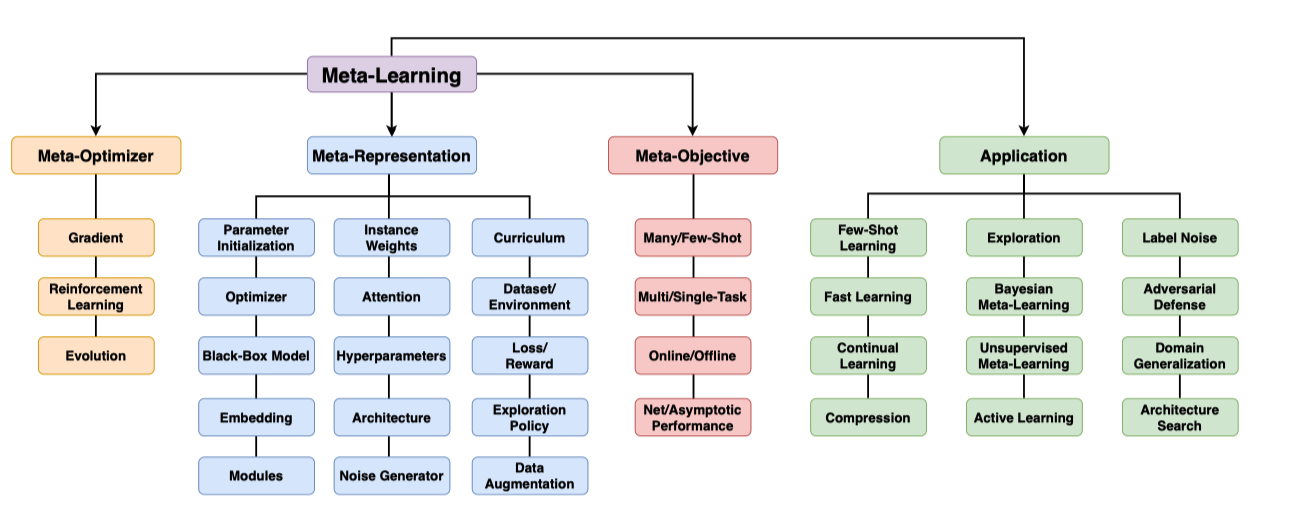
\includegraphics[width=1.1\textwidth]{figs/ml-landscape.png}}
}

%%//////////////////////////////////////////////////////////////////////////////////////////////%%58
\end{document}